%  !TeX  root  =  user_guide.tex

\section{Пространственный запрос}\label{sec:spatial_query}

% when the revision of a section has been finalized,
% comment out the following line:
% \updatedisclaimer

Модуль \toolbtntwo{spatialquery}{Пространственный запрос} позволяет выполнять
пространственные запросы (выделять объекты) к объектам целевого слоя по
отношению к объектам другого слоя. Модуль использует функционал библиотеки
GEOS (Geometry Engine "--- Open Source).

Поддерживаются следующие операторы:

\begin{itemize}[label=--]
\item Касается
\item Накладывается
\item Не пересекает
\item Пересекает
\item Пересекает кривой
\item Совпадает
\item Находится внутри
\end{itemize}

Не все типы геометрии поддерживают все перечисленные выше операторы.

\minisec{Работа с модулем}

В качестве примера найдем регионы Аляски, в которых есть аэропорт. Для этого:

\begin{enumerate}
\item Запустите \qg и загрузите слои \filename{regions.shp} и \filename{airports.shp}.
\item Активируйте модуль <<Пространственный запрос>> в Менеджере модулей
(см. Раздел~\ref{sec:load_core_plugin}) и нажмите на кнопку
\toolbtntwo{spatialquery}{Пространственный запрос} на панели инструментов.
Откроется окно, изображенное на рисунке~\ref{fig:spatialquerysample}.
\item Укажите слой regions в качестве исходного слоя, а слой в airports
как опорный слой.
\item Выберите оператор <<Содержит>> и нажмите \button{Применить}.
\end{enumerate}

В результате мы получим список идентификаторов объектов, удовлетворяющих
условию и можем.

\begin{itemize}[label=--]
\item \toolbtntwo{selectesubsetlayer}{Создать слой из выделенных объектов}
\item Выбрать идентификатор(ы) из списка и нажатием на \toolbtntwo{selectcreatelayer}{Создать слой из выделенных объектов}
\item Выбрать \button{Удалить из текущего выделения} группе <<Результат запроса>>.
\item Активировать флажок\checkbox{Увеличить до объекта} или отобразить \checkbox{Отладочные сообщения}.
\end{itemize}

\begin{figure}[ht]
   \centering
   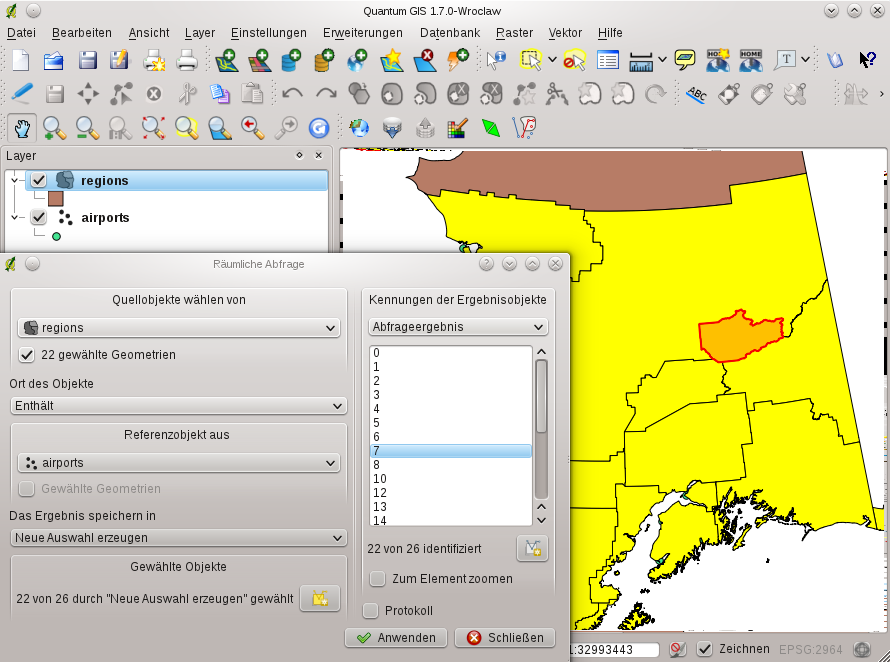
\includegraphics[clip=true, width=14cm]{spatial_query_sample}
   \caption{Пространственный запрос "--- области с аэропортами \nixcaption}
   \label{fig:spatialquerysample}
\end{figure}

\FloatBarrier

